\documentclass[]{article}
\usepackage{lmodern}
\usepackage{amssymb,amsmath}
\usepackage{ifxetex,ifluatex}
\usepackage{fixltx2e} % provides \textsubscript
\ifnum 0\ifxetex 1\fi\ifluatex 1\fi=0 % if pdftex
  \usepackage[T1]{fontenc}
  \usepackage[utf8]{inputenc}
\else % if luatex or xelatex
  \ifxetex
    \usepackage{mathspec}
  \else
    \usepackage{fontspec}
  \fi
  \defaultfontfeatures{Ligatures=TeX,Scale=MatchLowercase}
\fi
% use upquote if available, for straight quotes in verbatim environments
\IfFileExists{upquote.sty}{\usepackage{upquote}}{}
% use microtype if available
\IfFileExists{microtype.sty}{%
\usepackage{microtype}
\UseMicrotypeSet[protrusion]{basicmath} % disable protrusion for tt fonts
}{}
\usepackage[margin=1in]{geometry}
\usepackage{hyperref}
\hypersetup{unicode=true,
            pdftitle={PASS1A DMAQC data: analysis by BIC},
            pdfborder={0 0 0},
            breaklinks=true}
\urlstyle{same}  % don't use monospace font for urls
\usepackage{color}
\usepackage{fancyvrb}
\newcommand{\VerbBar}{|}
\newcommand{\VERB}{\Verb[commandchars=\\\{\}]}
\DefineVerbatimEnvironment{Highlighting}{Verbatim}{commandchars=\\\{\}}
% Add ',fontsize=\small' for more characters per line
\usepackage{framed}
\definecolor{shadecolor}{RGB}{248,248,248}
\newenvironment{Shaded}{\begin{snugshade}}{\end{snugshade}}
\newcommand{\KeywordTok}[1]{\textcolor[rgb]{0.13,0.29,0.53}{\textbf{#1}}}
\newcommand{\DataTypeTok}[1]{\textcolor[rgb]{0.13,0.29,0.53}{#1}}
\newcommand{\DecValTok}[1]{\textcolor[rgb]{0.00,0.00,0.81}{#1}}
\newcommand{\BaseNTok}[1]{\textcolor[rgb]{0.00,0.00,0.81}{#1}}
\newcommand{\FloatTok}[1]{\textcolor[rgb]{0.00,0.00,0.81}{#1}}
\newcommand{\ConstantTok}[1]{\textcolor[rgb]{0.00,0.00,0.00}{#1}}
\newcommand{\CharTok}[1]{\textcolor[rgb]{0.31,0.60,0.02}{#1}}
\newcommand{\SpecialCharTok}[1]{\textcolor[rgb]{0.00,0.00,0.00}{#1}}
\newcommand{\StringTok}[1]{\textcolor[rgb]{0.31,0.60,0.02}{#1}}
\newcommand{\VerbatimStringTok}[1]{\textcolor[rgb]{0.31,0.60,0.02}{#1}}
\newcommand{\SpecialStringTok}[1]{\textcolor[rgb]{0.31,0.60,0.02}{#1}}
\newcommand{\ImportTok}[1]{#1}
\newcommand{\CommentTok}[1]{\textcolor[rgb]{0.56,0.35,0.01}{\textit{#1}}}
\newcommand{\DocumentationTok}[1]{\textcolor[rgb]{0.56,0.35,0.01}{\textbf{\textit{#1}}}}
\newcommand{\AnnotationTok}[1]{\textcolor[rgb]{0.56,0.35,0.01}{\textbf{\textit{#1}}}}
\newcommand{\CommentVarTok}[1]{\textcolor[rgb]{0.56,0.35,0.01}{\textbf{\textit{#1}}}}
\newcommand{\OtherTok}[1]{\textcolor[rgb]{0.56,0.35,0.01}{#1}}
\newcommand{\FunctionTok}[1]{\textcolor[rgb]{0.00,0.00,0.00}{#1}}
\newcommand{\VariableTok}[1]{\textcolor[rgb]{0.00,0.00,0.00}{#1}}
\newcommand{\ControlFlowTok}[1]{\textcolor[rgb]{0.13,0.29,0.53}{\textbf{#1}}}
\newcommand{\OperatorTok}[1]{\textcolor[rgb]{0.81,0.36,0.00}{\textbf{#1}}}
\newcommand{\BuiltInTok}[1]{#1}
\newcommand{\ExtensionTok}[1]{#1}
\newcommand{\PreprocessorTok}[1]{\textcolor[rgb]{0.56,0.35,0.01}{\textit{#1}}}
\newcommand{\AttributeTok}[1]{\textcolor[rgb]{0.77,0.63,0.00}{#1}}
\newcommand{\RegionMarkerTok}[1]{#1}
\newcommand{\InformationTok}[1]{\textcolor[rgb]{0.56,0.35,0.01}{\textbf{\textit{#1}}}}
\newcommand{\WarningTok}[1]{\textcolor[rgb]{0.56,0.35,0.01}{\textbf{\textit{#1}}}}
\newcommand{\AlertTok}[1]{\textcolor[rgb]{0.94,0.16,0.16}{#1}}
\newcommand{\ErrorTok}[1]{\textcolor[rgb]{0.64,0.00,0.00}{\textbf{#1}}}
\newcommand{\NormalTok}[1]{#1}
\usepackage{graphicx,grffile}
\makeatletter
\def\maxwidth{\ifdim\Gin@nat@width>\linewidth\linewidth\else\Gin@nat@width\fi}
\def\maxheight{\ifdim\Gin@nat@height>\textheight\textheight\else\Gin@nat@height\fi}
\makeatother
% Scale images if necessary, so that they will not overflow the page
% margins by default, and it is still possible to overwrite the defaults
% using explicit options in \includegraphics[width, height, ...]{}
\setkeys{Gin}{width=\maxwidth,height=\maxheight,keepaspectratio}
\IfFileExists{parskip.sty}{%
\usepackage{parskip}
}{% else
\setlength{\parindent}{0pt}
\setlength{\parskip}{6pt plus 2pt minus 1pt}
}
\setlength{\emergencystretch}{3em}  % prevent overfull lines
\providecommand{\tightlist}{%
  \setlength{\itemsep}{0pt}\setlength{\parskip}{0pt}}
\setcounter{secnumdepth}{5}
% Redefines (sub)paragraphs to behave more like sections
\ifx\paragraph\undefined\else
\let\oldparagraph\paragraph
\renewcommand{\paragraph}[1]{\oldparagraph{#1}\mbox{}}
\fi
\ifx\subparagraph\undefined\else
\let\oldsubparagraph\subparagraph
\renewcommand{\subparagraph}[1]{\oldsubparagraph{#1}\mbox{}}
\fi

%%% Use protect on footnotes to avoid problems with footnotes in titles
\let\rmarkdownfootnote\footnote%
\def\footnote{\protect\rmarkdownfootnote}

%%% Change title format to be more compact
\usepackage{titling}

% Create subtitle command for use in maketitle
\newcommand{\subtitle}[1]{
  \posttitle{
    \begin{center}\large#1\end{center}
    }
}

\setlength{\droptitle}{-2em}
  \title{PASS1A DMAQC data: analysis by BIC}
  \pretitle{\vspace{\droptitle}\centering\huge}
  \posttitle{\par}
  \author{}
  \preauthor{}\postauthor{}
  \date{}
  \predate{}\postdate{}


\begin{document}
\maketitle

\begin{Shaded}
\begin{Highlighting}[]
\CommentTok{# Set the working directory to the folder with the data}
\NormalTok{dmaqc_data_dir =}\StringTok{ "/Users/David/Desktop/MoTrPAC/data/pass_1a/dmaqc_pheno/"}
\NormalTok{all_csvs =}\StringTok{ }\KeywordTok{list.files}\NormalTok{(dmaqc_data_dir,}\DataTypeTok{full.names =}\NormalTok{ T) }\CommentTok{# get all files in dir}
\NormalTok{all_csvs =}\StringTok{ }\NormalTok{all_csvs[}\KeywordTok{grepl}\NormalTok{(}\StringTok{".csv$"}\NormalTok{,all_csvs)] }\CommentTok{# make sure we take csv only}
\CommentTok{# read all files}
\NormalTok{csv_data =}\StringTok{ }\KeywordTok{list}\NormalTok{()}
\ControlFlowTok{for}\NormalTok{(fname }\ControlFlowTok{in}\NormalTok{ all_csvs)\{}
\NormalTok{  csv_data[[fname]] =}\StringTok{ }\KeywordTok{read.csv}\NormalTok{(fname,}\DataTypeTok{stringsAsFactors =}\NormalTok{ F)}
\NormalTok{\}}\CommentTok{# sapply(csv_data,dim) # check the dimensions of the different datasets}
\end{Highlighting}
\end{Shaded}

\section{Sanity check: Acute tests basic
statistics}\label{sanity-check-acute-tests-basic-statistics}

\begin{Shaded}
\begin{Highlighting}[]
\CommentTok{# Get the acute test data}
\NormalTok{ac_test_data =}\StringTok{ }\NormalTok{csv_data[[}\KeywordTok{which}\NormalTok{(}\KeywordTok{grepl}\NormalTok{(}\StringTok{"Acute.Test"}\NormalTok{,}\KeywordTok{names}\NormalTok{(csv_data)))]]}
\KeywordTok{dim}\NormalTok{(ac_test_data)}
\end{Highlighting}
\end{Shaded}

\begin{verbatim}
## [1] 108  23
\end{verbatim}

\begin{Shaded}
\begin{Highlighting}[]
\CommentTok{# check the time differences between start and end}
\NormalTok{test_times =}\StringTok{ }\KeywordTok{as.difftime}\NormalTok{(ac_test_data}\OperatorTok{$}\NormalTok{t_complete) }\OperatorTok{-}\StringTok{ }\KeywordTok{as.difftime}\NormalTok{(ac_test_data}\OperatorTok{$}\NormalTok{t_start)}
\CommentTok{# table of the values: all except for on are 0.5 hours}
\KeywordTok{table}\NormalTok{(test_times)}
\end{Highlighting}
\end{Shaded}

\begin{verbatim}
## test_times
## 0.466666666666667               0.5 
##                 1               107
\end{verbatim}

\begin{Shaded}
\begin{Highlighting}[]
\CommentTok{# Get the comment of the sample that is not 0.5h}
\NormalTok{ac_test_data[test_times}\OperatorTok{!=}\FloatTok{0.5}\NormalTok{,}\StringTok{"comments"}\NormalTok{]}
\end{Highlighting}
\end{Shaded}

\begin{verbatim}
## [1] "Treadmill stopped 28:49 (mm:ss) into the acute bout due to problems with the other rat on the same treadmill."
\end{verbatim}

\begin{Shaded}
\begin{Highlighting}[]
\NormalTok{ac_test_data}\OperatorTok{$}\NormalTok{formatted_test_time =}\StringTok{ }\NormalTok{test_times}
\end{Highlighting}
\end{Shaded}

Next, we analyze the distances. We illustrate how these are a function
of the shocks and sex/weight.

\begin{Shaded}
\begin{Highlighting}[]
\CommentTok{# convert the shock lengths to numbers (seconds)}
\NormalTok{parse_shocktime<-}\ControlFlowTok{function}\NormalTok{(x)\{}
\NormalTok{  arr =}\StringTok{ }\KeywordTok{strsplit}\NormalTok{(x,}\DataTypeTok{split=}\StringTok{":"}\NormalTok{)[[}\DecValTok{1}\NormalTok{]]}
  \ControlFlowTok{if}\NormalTok{(}\KeywordTok{length}\NormalTok{(arr)}\OperatorTok{<}\DecValTok{2}\NormalTok{)\{}\KeywordTok{return}\NormalTok{(}\OtherTok{NA}\NormalTok{)\}}
  \KeywordTok{return}\NormalTok{(}\KeywordTok{as.numeric}\NormalTok{(arr[}\DecValTok{1}\NormalTok{])}\OperatorTok{*}\DecValTok{60}\OperatorTok{+}\KeywordTok{as.numeric}\NormalTok{(arr[}\DecValTok{2}\NormalTok{]))}
\NormalTok{\}}
\NormalTok{tmp_x =}\StringTok{ }\NormalTok{ac_test_data}\OperatorTok{$}\NormalTok{howlongshock}
\NormalTok{tmp_x =}\StringTok{ }\KeywordTok{sapply}\NormalTok{(tmp_x, parse_shocktime)}
\NormalTok{ac_test_data}\OperatorTok{$}\NormalTok{howlongshock =}\StringTok{ }\NormalTok{tmp_x}
\KeywordTok{rm}\NormalTok{(tmp_x)}

\KeywordTok{par}\NormalTok{(}\DataTypeTok{mfrow=}\KeywordTok{c}\NormalTok{(}\DecValTok{1}\NormalTok{,}\DecValTok{2}\NormalTok{))}
\CommentTok{# histogram of distances}
\KeywordTok{hist}\NormalTok{(ac_test_data}\OperatorTok{$}\NormalTok{distance,}\DataTypeTok{col=}\StringTok{"blue"}\NormalTok{,}\DataTypeTok{breaks=}\DecValTok{50}\NormalTok{,}\DataTypeTok{main =} \StringTok{"Histogram of distances"}\NormalTok{)}

\CommentTok{# Correlation between distance and number of shocks}
\CommentTok{# Get the indices of the samples with shock information -}
\CommentTok{# these the animals that did the acute test}
\NormalTok{timesshock_inds =}\StringTok{ }\OperatorTok{!}\KeywordTok{is.na}\NormalTok{(ac_test_data}\OperatorTok{$}\NormalTok{timesshock)}
\CommentTok{# create a new dataframe with the selected animals}
\NormalTok{trained_animals_data =}\StringTok{ }\NormalTok{ac_test_data[timesshock_inds,]}
\NormalTok{sp_corr =}\StringTok{ }\KeywordTok{cor}\NormalTok{(trained_animals_data}\OperatorTok{$}\NormalTok{distance,}
\NormalTok{              trained_animals_data}\OperatorTok{$}\NormalTok{timesshock,}\DataTypeTok{method=}\StringTok{"spearman"}\NormalTok{)}
\KeywordTok{plot}\NormalTok{(trained_animals_data}\OperatorTok{$}\NormalTok{distance,trained_animals_data}\OperatorTok{$}\NormalTok{timesshock,}
     \DataTypeTok{main=}\KeywordTok{paste}\NormalTok{(}\StringTok{"Dist vs times shocked, rho="}\NormalTok{,}\KeywordTok{format}\NormalTok{(sp_corr,}\DataTypeTok{digits =} \DecValTok{2}\NormalTok{),}\DataTypeTok{sep=}\StringTok{""}\NormalTok{),}
     \DataTypeTok{pch=}\DecValTok{20}\NormalTok{,}\DataTypeTok{ylab=}\StringTok{"Times shock given"}\NormalTok{,}\DataTypeTok{xlab=}\StringTok{"Distance"}\NormalTok{,}\DataTypeTok{cex.main=}\FloatTok{1.1}\NormalTok{)}
\end{Highlighting}
\end{Shaded}

\begin{center}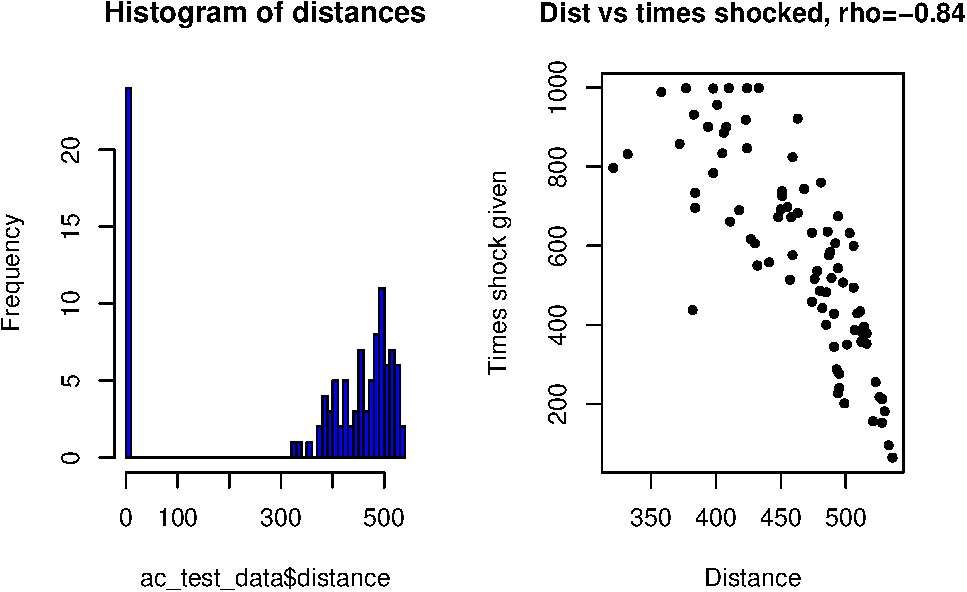
\includegraphics[width=0.6\linewidth,height=0.6\textheight]{pheno_csv_files_analysis_files/figure-latex/unnamed-chunk-3-1} \end{center}

\begin{Shaded}
\begin{Highlighting}[]
\CommentTok{# A "smarter" analysis: regression of the distance using shock info}
\NormalTok{dist_lm  =}\StringTok{ }\KeywordTok{lm}\NormalTok{(distance}\OperatorTok{~}\NormalTok{timesshock}\OperatorTok{+}\NormalTok{howlongshock}\OperatorTok{+}\NormalTok{weight}\OperatorTok{+}\NormalTok{days_start,}
              \DataTypeTok{data=}\NormalTok{trained_animals_data)}
\CommentTok{# Summary of the model, points to take: high R^2, significance of}
\CommentTok{# the features}
\KeywordTok{summary}\NormalTok{(dist_lm)}
\end{Highlighting}
\end{Shaded}

\begin{verbatim}
## 
## Call:
## lm(formula = distance ~ timesshock + howlongshock + weight + 
##     days_start, data = trained_animals_data)
## 
## Residuals:
##      Min       1Q   Median       3Q      Max 
## -22.1248  -1.0430   0.6867   2.4416   8.8814 
## 
## Coefficients:
##                Estimate Std. Error t value Pr(>|t|)    
## (Intercept)  562.127804   2.427681 231.549   <2e-16 ***
## timesshock     0.003171   0.003464   0.916    0.363    
## howlongshock  -0.296415   0.005700 -52.004   <2e-16 ***
## weight        -0.147827   0.006563 -22.526   <2e-16 ***
## days_start     0.032731   0.024534   1.334    0.186    
## ---
## Signif. codes:  0 '***' 0.001 '**' 0.01 '*' 0.05 '.' 0.1 ' ' 1
## 
## Residual standard error: 4.623 on 79 degrees of freedom
## Multiple R-squared:  0.9921, Adjusted R-squared:  0.9917 
## F-statistic:  2466 on 4 and 79 DF,  p-value: < 2.2e-16
\end{verbatim}

\begin{Shaded}
\begin{Highlighting}[]
\CommentTok{# We have some clear outliers:}
\KeywordTok{library}\NormalTok{(MASS)}
\KeywordTok{par}\NormalTok{(}\DataTypeTok{mfrow=}\KeywordTok{c}\NormalTok{(}\DecValTok{1}\NormalTok{,}\DecValTok{2}\NormalTok{))}
\KeywordTok{plot}\NormalTok{(}\KeywordTok{studres}\NormalTok{(dist_lm),}\DataTypeTok{main=}\StringTok{"studentized residuals (lm)"}\NormalTok{,}\DataTypeTok{ylab=}\StringTok{"residual"}\NormalTok{)}
\CommentTok{# Select the top outliers and look at their comments}
\NormalTok{outliers =}\StringTok{ }\KeywordTok{abs}\NormalTok{(}\KeywordTok{studres}\NormalTok{(dist_lm)) }\OperatorTok{>}\StringTok{ }\DecValTok{2}
\CommentTok{# how many outliers have we selected?}
\KeywordTok{sum}\NormalTok{(outliers)}
\end{Highlighting}
\end{Shaded}

\begin{verbatim}
## [1] 4
\end{verbatim}

\begin{Shaded}
\begin{Highlighting}[]
\CommentTok{# their comments:}
\NormalTok{trained_animals_data[outliers,}\StringTok{"comments"}\NormalTok{]}
\end{Highlighting}
\end{Shaded}

\begin{verbatim}
## [1] "Increased shock at 20 min."                                                                                                                     
## [2] "Treadmill stopped 28:49 (mm:ss) into the acute bout due to problems with the other rat on the same treadmill."                                  
## [3] "Shock grid increased to 1.0 mA at 22 minutes. Treadmill bout stopped at 28:49 (mm:ss) due to animal distress and inability to continue running."
## [4] ""
\end{verbatim}

\begin{Shaded}
\begin{Highlighting}[]
\CommentTok{# Plot the fitted values of the linear regression vs.}
\CommentTok{# the true distances}
\KeywordTok{plot}\NormalTok{(dist_lm}\OperatorTok{$}\NormalTok{fitted.values,trained_animals_data}\OperatorTok{$}\NormalTok{distance,}\DataTypeTok{lwd=}\DecValTok{2}\NormalTok{,}
     \DataTypeTok{main=}\StringTok{"Fitted vs real values"}\NormalTok{,}\DataTypeTok{ylab=}\StringTok{"Distances"}\NormalTok{,}\DataTypeTok{xlab=}\StringTok{"Fitted distances"}\NormalTok{)}
\KeywordTok{abline}\NormalTok{(}\DecValTok{0}\NormalTok{,}\DecValTok{1}\NormalTok{,}\DataTypeTok{col=}\StringTok{"red"}\NormalTok{,}\DataTypeTok{lty=}\DecValTok{2}\NormalTok{,}\DataTypeTok{lwd=}\DecValTok{3}\NormalTok{)}
\end{Highlighting}
\end{Shaded}

\begin{center}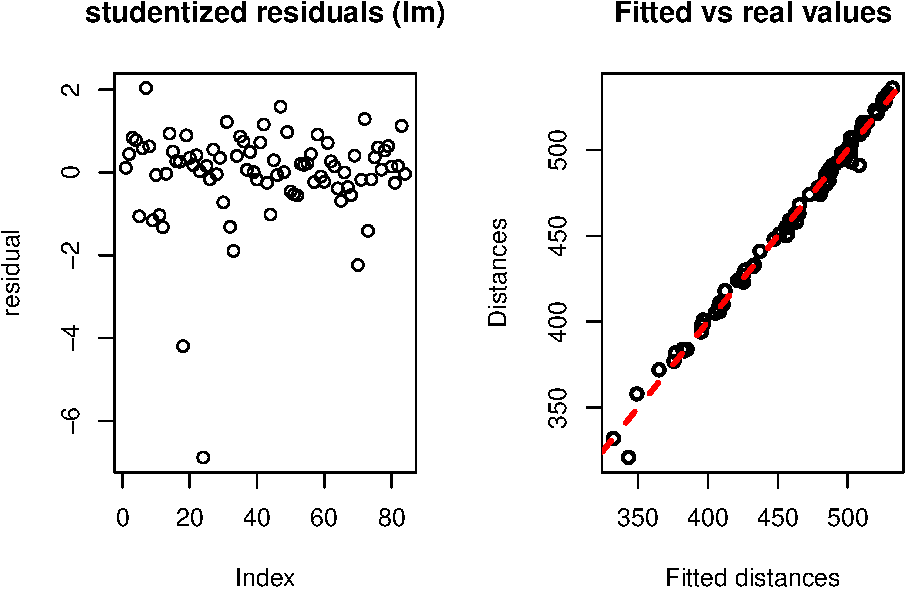
\includegraphics[width=0.6\linewidth,height=0.6\textheight]{pheno_csv_files_analysis_files/figure-latex/unnamed-chunk-3-2} \end{center}

\section{Site comparison}\label{site-comparison}

In some versions of the DMAQC data there is a single site. In this case
this section will not result in an output.

\begin{Shaded}
\begin{Highlighting}[]
\CommentTok{# Load additional information about the animals}
\NormalTok{registr_data =}\StringTok{ }\NormalTok{csv_data[[}\KeywordTok{which}\NormalTok{(}\KeywordTok{grepl}\NormalTok{(}\StringTok{"Regist"}\NormalTok{,}\KeywordTok{names}\NormalTok{(csv_data)))]]}
\KeywordTok{rownames}\NormalTok{(registr_data) =}\StringTok{ }\KeywordTok{as.character}\NormalTok{(registr_data}\OperatorTok{$}\NormalTok{pid)}
\CommentTok{# make the rownames in the test data comparable}
\KeywordTok{rownames}\NormalTok{(trained_animals_data) =}\StringTok{ }\NormalTok{trained_animals_data}\OperatorTok{$}\NormalTok{pid}
\CommentTok{# add sex to the trained animal data data frame}
\NormalTok{sex_key =}\StringTok{ }\KeywordTok{c}\NormalTok{(}\StringTok{"Female"}\NormalTok{,}\StringTok{"Male"}\NormalTok{)}
\NormalTok{trained_animals_data}\OperatorTok{$}\NormalTok{sex =}\StringTok{ }\NormalTok{sex_key[registr_data[}\KeywordTok{rownames}\NormalTok{(trained_animals_data),}\StringTok{"sex"}\NormalTok{]]}

\CommentTok{# Map site Ids to their names}
\NormalTok{site_names =}\StringTok{ }\KeywordTok{c}\NormalTok{(}\StringTok{"910"}\NormalTok{=}\StringTok{"Joslin"}\NormalTok{,}\StringTok{"930"}\NormalTok{=}\StringTok{"Florida"}\NormalTok{)}
\NormalTok{trained_animals_data}\OperatorTok{$}\NormalTok{site =}\StringTok{ }\NormalTok{site_names[}\KeywordTok{as.character}\NormalTok{(trained_animals_data}\OperatorTok{$}\NormalTok{siteID)]}

\CommentTok{# Sanity check: the numbers should be the same for both sites}
\KeywordTok{table}\NormalTok{(ac_test_data}\OperatorTok{$}\NormalTok{siteID)}
\end{Highlighting}
\end{Shaded}

\begin{verbatim}
## 
## 910 
## 108
\end{verbatim}

\begin{Shaded}
\begin{Highlighting}[]
\KeywordTok{table}\NormalTok{(trained_animals_data}\OperatorTok{$}\NormalTok{site,trained_animals_data}\OperatorTok{$}\NormalTok{sex)}
\end{Highlighting}
\end{Shaded}

\begin{verbatim}
##         
##          Female Male
##   Joslin     42   42
\end{verbatim}

\begin{Shaded}
\begin{Highlighting}[]
\NormalTok{run_wilcox<-}\ControlFlowTok{function}\NormalTok{(x1,x2)\{}
  \KeywordTok{return}\NormalTok{(}\KeywordTok{wilcox.test}\NormalTok{(x1[x2}\OperatorTok{==}\NormalTok{x2[}\DecValTok{1}\NormalTok{]],x1[x2}\OperatorTok{!=}\NormalTok{x2[}\DecValTok{1}\NormalTok{]])}\OperatorTok{$}\NormalTok{p.value)}
\NormalTok{\}}
\CommentTok{# Compare the distances, shocks, and weight (if we have multiple site)}
\ControlFlowTok{if}\NormalTok{ (}\KeywordTok{length}\NormalTok{(}\KeywordTok{unique}\NormalTok{(ac_test_data}\OperatorTok{$}\NormalTok{siteID))}\OperatorTok{>}\DecValTok{1}\NormalTok{)\{}
  \KeywordTok{par}\NormalTok{(}\DataTypeTok{mfrow=}\KeywordTok{c}\NormalTok{(}\DecValTok{1}\NormalTok{,}\DecValTok{3}\NormalTok{),}\DataTypeTok{mar=}\KeywordTok{c}\NormalTok{(}\DecValTok{10}\NormalTok{,}\DecValTok{4}\NormalTok{,}\DecValTok{4}\NormalTok{,}\DecValTok{4}\NormalTok{))}
  \CommentTok{# Site only}
\NormalTok{  p_dist =}\StringTok{ }\KeywordTok{run_wilcox}\NormalTok{(trained_animals_data}\OperatorTok{$}\NormalTok{distance,trained_animals_data}\OperatorTok{$}\NormalTok{site)}
  \KeywordTok{boxplot}\NormalTok{(distance}\OperatorTok{~}\NormalTok{site,}\DataTypeTok{data=}\NormalTok{trained_animals_data,}\DataTypeTok{col=}\StringTok{"cyan"}\NormalTok{,}\DataTypeTok{ylab=}\StringTok{"Distance"}\NormalTok{,}
        \DataTypeTok{main=}\KeywordTok{paste}\NormalTok{(}\StringTok{"Site vs. distance, p<"}\NormalTok{,}\KeywordTok{format}\NormalTok{(p_dist,}\DataTypeTok{digits =} \DecValTok{2}\NormalTok{)),}
        \DataTypeTok{cex.main=}\DecValTok{1}\NormalTok{,}\DataTypeTok{las=}\DecValTok{2}\NormalTok{)}
\NormalTok{  p_timesshock =}\StringTok{ }\KeywordTok{run_wilcox}\NormalTok{(trained_animals_data}\OperatorTok{$}\NormalTok{timesshock,trained_animals_data}\OperatorTok{$}\NormalTok{site)}
  \KeywordTok{boxplot}\NormalTok{(timesshock}\OperatorTok{~}\NormalTok{site,}\DataTypeTok{data=}\NormalTok{trained_animals_data,}\DataTypeTok{col=}\StringTok{"red"}\NormalTok{,}\DataTypeTok{ylab=}\StringTok{"Times shocked"}\NormalTok{,}
        \DataTypeTok{main=}\KeywordTok{paste}\NormalTok{(}\StringTok{"Site vs. times shocked, p<"}\NormalTok{,}\KeywordTok{format}\NormalTok{(p_timesshock,}\DataTypeTok{digits =} \DecValTok{3}\NormalTok{)),}
        \DataTypeTok{cex.main=}\DecValTok{1}\NormalTok{,}\DataTypeTok{las=}\DecValTok{2}\NormalTok{)}
\NormalTok{  p_w =}\StringTok{ }\KeywordTok{run_wilcox}\NormalTok{(trained_animals_data}\OperatorTok{$}\NormalTok{weight,trained_animals_data}\OperatorTok{$}\NormalTok{site)}
  \KeywordTok{boxplot}\NormalTok{(weight}\OperatorTok{~}\NormalTok{site,}\DataTypeTok{data=}\NormalTok{trained_animals_data,}\DataTypeTok{col=}\StringTok{"cyan"}\NormalTok{,}\DataTypeTok{ylab=}\StringTok{"Weight"}\NormalTok{,}
        \DataTypeTok{main=}\KeywordTok{paste}\NormalTok{(}\StringTok{"Site vs. weight, p="}\NormalTok{,}\KeywordTok{format}\NormalTok{(p_w,}\DataTypeTok{digits =} \DecValTok{2}\NormalTok{)),}
        \DataTypeTok{cex.main=}\DecValTok{1}\NormalTok{,}\DataTypeTok{las=}\DecValTok{2}\NormalTok{)}
  \CommentTok{# Site and sex}
  \KeywordTok{par}\NormalTok{(}\DataTypeTok{mfrow=}\KeywordTok{c}\NormalTok{(}\DecValTok{1}\NormalTok{,}\DecValTok{3}\NormalTok{),}\DataTypeTok{mar=}\KeywordTok{c}\NormalTok{(}\DecValTok{10}\NormalTok{,}\DecValTok{4}\NormalTok{,}\DecValTok{4}\NormalTok{,}\DecValTok{4}\NormalTok{))}
  \KeywordTok{boxplot}\NormalTok{(distance}\OperatorTok{~}\NormalTok{site}\OperatorTok{+}\NormalTok{sex,}\DataTypeTok{data=}\NormalTok{trained_animals_data,}\DataTypeTok{col=}\StringTok{"cyan"}\NormalTok{,}\DataTypeTok{ylab=}\StringTok{"Distance"}\NormalTok{,}
        \DataTypeTok{main=}\StringTok{"Site vs. distance"}\NormalTok{,}\DataTypeTok{cex.main=}\DecValTok{1}\NormalTok{,}\DataTypeTok{las=}\DecValTok{2}\NormalTok{)}
  \KeywordTok{boxplot}\NormalTok{(timesshock}\OperatorTok{~}\NormalTok{site}\OperatorTok{+}\NormalTok{sex,}\DataTypeTok{data=}\NormalTok{trained_animals_data,}\DataTypeTok{col=}\StringTok{"red"}\NormalTok{,}\DataTypeTok{ylab=}\StringTok{"Times shocked"}\NormalTok{,}
        \DataTypeTok{main=}\StringTok{"Site vs. times shocked"}\NormalTok{,}\DataTypeTok{cex.main=}\DecValTok{1}\NormalTok{,}\DataTypeTok{las=}\DecValTok{2}\NormalTok{)}
  \KeywordTok{boxplot}\NormalTok{(weight}\OperatorTok{~}\NormalTok{site}\OperatorTok{+}\NormalTok{sex,}\DataTypeTok{data=}\NormalTok{trained_animals_data,}\DataTypeTok{col=}\StringTok{"cyan"}\NormalTok{,}\DataTypeTok{ylab=}\StringTok{"Weight"}\NormalTok{,}
        \DataTypeTok{main=}\StringTok{"Site vs. weight"}\NormalTok{,}\DataTypeTok{cex.main=}\DecValTok{1}\NormalTok{,}\DataTypeTok{las=}\DecValTok{2}\NormalTok{)}

  \CommentTok{# Regress time shocked and distance vs. site and sex}
  \KeywordTok{summary}\NormalTok{(}\KeywordTok{lm}\NormalTok{(timesshock}\OperatorTok{~}\NormalTok{site}\OperatorTok{+}\NormalTok{sex,}\DataTypeTok{data=}\NormalTok{trained_animals_data))}
  \KeywordTok{summary}\NormalTok{(}\KeywordTok{lm}\NormalTok{(distance}\OperatorTok{~}\NormalTok{site}\OperatorTok{+}\NormalTok{sex,}\DataTypeTok{data=}\NormalTok{trained_animals_data))  }
\NormalTok{  \}}
\end{Highlighting}
\end{Shaded}

\section{Sanity checks: Biospecimen
data}\label{sanity-checks-biospecimen-data}

\begin{Shaded}
\begin{Highlighting}[]
\CommentTok{# Analysis of biospecimen data}
\NormalTok{spec_data =}\StringTok{ }\NormalTok{csv_data[[}\KeywordTok{which}\NormalTok{(}\KeywordTok{grepl}\NormalTok{(}\StringTok{"Specimen.Processing.csv"}\NormalTok{,}\KeywordTok{names}\NormalTok{(csv_data)))]]}
\KeywordTok{rownames}\NormalTok{(spec_data) =}\StringTok{ }\NormalTok{spec_data}\OperatorTok{$}\NormalTok{labelid}
\CommentTok{# Parse the times and compute the difference between the freeze time and }
\CommentTok{# the collection time}
\NormalTok{time_to_freeze1 =}\StringTok{ }\KeywordTok{as.difftime}\NormalTok{(spec_data}\OperatorTok{$}\NormalTok{t_freeze,}\DataTypeTok{units =} \StringTok{"mins"}\NormalTok{) }\OperatorTok{-}
\StringTok{  }\KeywordTok{as.difftime}\NormalTok{(spec_data}\OperatorTok{$}\NormalTok{t_collection,}\DataTypeTok{units=}\StringTok{"mins"}\NormalTok{)}
\CommentTok{# For some samples we have the edta spin time instead of the collection}
\CommentTok{# time, use these when there are no other options}
\NormalTok{time_to_freeze2 =}\StringTok{ }\KeywordTok{as.difftime}\NormalTok{(spec_data}\OperatorTok{$}\NormalTok{t_freeze,}\DataTypeTok{units =} \StringTok{"mins"}\NormalTok{) }\OperatorTok{-}
\StringTok{  }\KeywordTok{as.difftime}\NormalTok{(spec_data}\OperatorTok{$}\NormalTok{t_edtaspin,}\DataTypeTok{units=}\StringTok{"mins"}\NormalTok{)}
\NormalTok{time_to_freeze =}\StringTok{ }\NormalTok{time_to_freeze1}
\CommentTok{# Fill in the NAs by taking the time between the edta spin and the freeze}
\KeywordTok{table}\NormalTok{(}\KeywordTok{is.na}\NormalTok{(time_to_freeze1),}\KeywordTok{is.na}\NormalTok{(time_to_freeze2))}
\end{Highlighting}
\end{Shaded}

\begin{verbatim}
##        
##         FALSE TRUE
##   FALSE     0 2182
##   TRUE    517    0
\end{verbatim}

\begin{Shaded}
\begin{Highlighting}[]
\NormalTok{time_to_freeze[}\KeywordTok{is.na}\NormalTok{(time_to_freeze1)] =}\StringTok{ }\NormalTok{time_to_freeze2[}\KeywordTok{is.na}\NormalTok{(time_to_freeze1)]}
\NormalTok{spec_data}\OperatorTok{$}\NormalTok{time_to_freeze =}\StringTok{ }\KeywordTok{as.numeric}\NormalTok{(time_to_freeze)}
\NormalTok{spec_data}\OperatorTok{$}\NormalTok{time_to_freeze_from_collection =}\StringTok{ }\KeywordTok{as.numeric}\NormalTok{(time_to_freeze1)}
\NormalTok{spec_data}\OperatorTok{$}\NormalTok{time_to_freeze_from_edta_spin =}\StringTok{ }\KeywordTok{as.numeric}\NormalTok{(time_to_freeze2)}
\KeywordTok{hist}\NormalTok{(spec_data}\OperatorTok{$}\NormalTok{time_to_freeze,}\DataTypeTok{breaks =} \DecValTok{100}\NormalTok{)}
\end{Highlighting}
\end{Shaded}

\begin{center}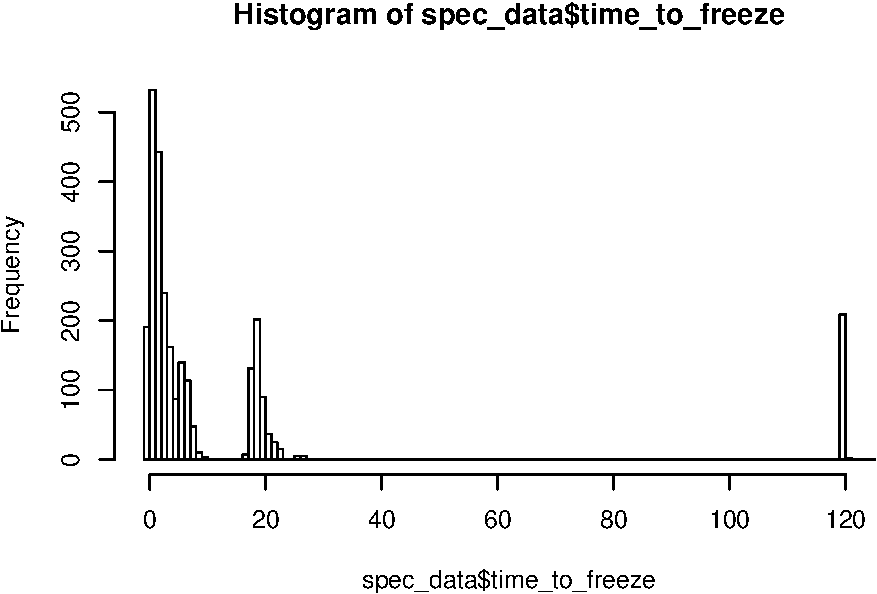
\includegraphics[width=0.5\linewidth,height=0.5\textheight]{pheno_csv_files_analysis_files/figure-latex/unnamed-chunk-5-1} \end{center}

\begin{Shaded}
\begin{Highlighting}[]
\CommentTok{# Add site by name}
\NormalTok{site_names =}\StringTok{ }\KeywordTok{c}\NormalTok{(}\StringTok{"910"}\NormalTok{=}\StringTok{"Joslin"}\NormalTok{,}\StringTok{"930"}\NormalTok{=}\StringTok{"Florida"}\NormalTok{)}
\NormalTok{spec_data}\OperatorTok{$}\NormalTok{site =}\StringTok{ }\NormalTok{site_names[}\KeywordTok{as.character}\NormalTok{(spec_data}\OperatorTok{$}\NormalTok{siteid)]}
\KeywordTok{table}\NormalTok{(spec_data}\OperatorTok{$}\NormalTok{site)}
\end{Highlighting}
\end{Shaded}

\begin{verbatim}
## 
## Joslin 
##   2699
\end{verbatim}

\begin{Shaded}
\begin{Highlighting}[]
\NormalTok{inds =}\StringTok{ }\OperatorTok{!}\KeywordTok{is.na}\NormalTok{(time_to_freeze1)}
\NormalTok{inds =}\StringTok{ }\KeywordTok{grepl}\NormalTok{(}\StringTok{"adipose"}\NormalTok{,spec_data}\OperatorTok{$}\NormalTok{sampletypedescription,}\DataTypeTok{ignore.case =}\NormalTok{ T)}
\NormalTok{inds =}\StringTok{ }\KeywordTok{grepl}\NormalTok{(}\StringTok{"heart"}\NormalTok{,spec_data}\OperatorTok{$}\NormalTok{sampletypedescription,}\DataTypeTok{ignore.case =}\NormalTok{ T) }\OperatorTok{|}\StringTok{ }
\StringTok{  }\KeywordTok{grepl}\NormalTok{(}\StringTok{"liver"}\NormalTok{,spec_data}\OperatorTok{$}\NormalTok{sampletypedescription,}\DataTypeTok{ignore.case =}\NormalTok{ T) }\OperatorTok{|}
\StringTok{  }\KeywordTok{grepl}\NormalTok{(}\StringTok{"colon"}\NormalTok{,spec_data}\OperatorTok{$}\NormalTok{sampletypedescription,}\DataTypeTok{ignore.case =}\NormalTok{ T) }\OperatorTok{|}\StringTok{ }
\StringTok{  }\KeywordTok{grepl}\NormalTok{(}\StringTok{"vastus"}\NormalTok{,spec_data}\OperatorTok{$}\NormalTok{sampletypedescription,}\DataTypeTok{ignore.case =}\NormalTok{ T)}
\CommentTok{# Using site info:}
\CommentTok{# Here we use an interaction term and not addition as the R^2 is >2 times}
\CommentTok{# greater this way}
\ControlFlowTok{if}\NormalTok{ (}\KeywordTok{length}\NormalTok{(}\KeywordTok{unique}\NormalTok{(spec_data}\OperatorTok{$}\NormalTok{site))}\OperatorTok{>}\DecValTok{1}\NormalTok{)\{}
  \KeywordTok{par}\NormalTok{(}\DataTypeTok{mar=}\KeywordTok{c}\NormalTok{(}\DecValTok{10}\NormalTok{,}\DecValTok{2}\NormalTok{,}\DecValTok{2}\NormalTok{,}\DecValTok{2}\NormalTok{))}
  \KeywordTok{boxplot}\NormalTok{(time_to_freeze}\OperatorTok{~}\NormalTok{site}\OperatorTok{:}\NormalTok{sampletypedescription,}\DataTypeTok{data=}\NormalTok{spec_data[inds,],}
        \DataTypeTok{ylab=}\StringTok{"Time to freeze"}\NormalTok{,}\DataTypeTok{las=}\DecValTok{2}\NormalTok{)  }
  \KeywordTok{summary}\NormalTok{(}\KeywordTok{lm}\NormalTok{(time_to_freeze}\OperatorTok{~}\NormalTok{sampletypedescription}\OperatorTok{:}\NormalTok{site,}\DataTypeTok{data=}\NormalTok{spec_data[inds,]))}
\NormalTok{\}}
\CommentTok{# A single site}
\ControlFlowTok{if}\NormalTok{ (}\KeywordTok{length}\NormalTok{(}\KeywordTok{unique}\NormalTok{(spec_data}\OperatorTok{$}\NormalTok{site))}\OperatorTok{==}\DecValTok{1}\NormalTok{)\{}
  \KeywordTok{par}\NormalTok{(}\DataTypeTok{mar=}\KeywordTok{c}\NormalTok{(}\DecValTok{10}\NormalTok{,}\DecValTok{2}\NormalTok{,}\DecValTok{2}\NormalTok{,}\DecValTok{2}\NormalTok{))}
  \KeywordTok{boxplot}\NormalTok{(time_to_freeze}\OperatorTok{~}\NormalTok{sampletypedescription,}\DataTypeTok{data=}\NormalTok{spec_data[inds,],}
        \DataTypeTok{ylab=}\StringTok{"Time to freeze"}\NormalTok{,}\DataTypeTok{las=}\DecValTok{2}\NormalTok{)  }
  \KeywordTok{summary}\NormalTok{(}\KeywordTok{lm}\NormalTok{(time_to_freeze}\OperatorTok{~}\NormalTok{sampletypedescription,}\DataTypeTok{data=}\NormalTok{spec_data[inds,]))}
\NormalTok{\}}
\end{Highlighting}
\end{Shaded}

\begin{center}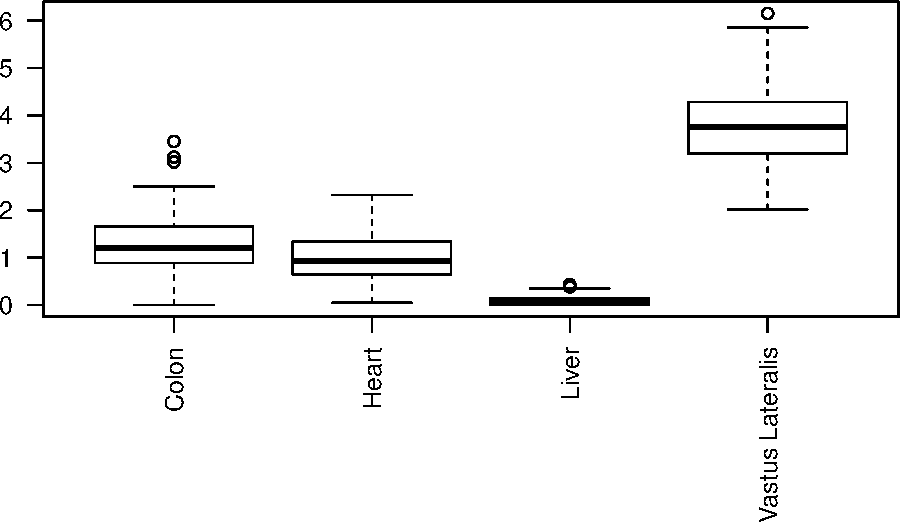
\includegraphics[width=0.5\linewidth,height=0.5\textheight]{pheno_csv_files_analysis_files/figure-latex/unnamed-chunk-5-2} \end{center}

\begin{verbatim}
## 
## Call:
## lm(formula = time_to_freeze ~ sampletypedescription, data = spec_data[inds, 
##     ])
## 
## Residuals:
##      Min       1Q   Median       3Q      Max 
## -1.78765 -0.33731 -0.05216  0.27994  2.34568 
## 
## Coefficients:
##                                       Estimate Std. Error t value Pr(>|t|)
## (Intercept)                            1.32052    0.05478  24.106  < 2e-16
## sampletypedescriptionHeart            -0.30046    0.07747  -3.878 0.000122
## sampletypedescriptionLiver            -1.23503    0.07747 -15.942  < 2e-16
## sampletypedescriptionVastus Lateralis  2.48380    0.07747  32.061  < 2e-16
##                                          
## (Intercept)                           ***
## sampletypedescriptionHeart            ***
## sampletypedescriptionLiver            ***
## sampletypedescriptionVastus Lateralis ***
## ---
## Signif. codes:  0 '***' 0.001 '**' 0.01 '*' 0.05 '.' 0.1 ' ' 1
## 
## Residual standard error: 0.5693 on 428 degrees of freedom
## Multiple R-squared:  0.8548, Adjusted R-squared:  0.8538 
## F-statistic: 839.8 on 3 and 428 DF,  p-value: < 2.2e-16
\end{verbatim}

\section{Format the metadata table according to vial
ids}\label{format-the-metadata-table-according-to-vial-ids}

We now use DMAQC's mapping of label ids to vial ids and use it to
generate a single metadata table that we can share with other sites.

\begin{Shaded}
\begin{Highlighting}[]
\CommentTok{# Helper function for merging columns from data2 into data1}
\NormalTok{merge_avoid_col_dup<-}\ControlFlowTok{function}\NormalTok{(data1,data2,by_col)\{}
\NormalTok{  data2_cols =}\StringTok{ }\KeywordTok{c}\NormalTok{(by_col,}\KeywordTok{setdiff}\NormalTok{(}\KeywordTok{colnames}\NormalTok{(data2),}\KeywordTok{colnames}\NormalTok{(data1)))}
  \KeywordTok{return}\NormalTok{(}\KeywordTok{merge}\NormalTok{(data1, data2[,data2_cols], }\DataTypeTok{by=}\NormalTok{by_col))}
\NormalTok{\}}
\CommentTok{# Get the animal data and merge}
\NormalTok{merged_animal_data =}\StringTok{ }\NormalTok{ac_test_data}
\KeywordTok{colnames}\NormalTok{(merged_animal_data) =}\StringTok{ }\KeywordTok{paste}\NormalTok{(}\StringTok{"Acute.test"}\NormalTok{,}\KeywordTok{colnames}\NormalTok{(merged_animal_data),}\DataTypeTok{sep=}\StringTok{"_"}\NormalTok{)}
\KeywordTok{colnames}\NormalTok{(merged_animal_data)[}\KeywordTok{grepl}\NormalTok{(}\StringTok{"_pid$"}\NormalTok{,}\KeywordTok{colnames}\NormalTok{(merged_animal_data))]=}\StringTok{"pid"}
\NormalTok{tmp_ac_data =}\StringTok{ }\NormalTok{csv_data[[}\KeywordTok{which}\NormalTok{(}\KeywordTok{grepl}\NormalTok{(}\StringTok{"Animal.Familiarization"}\NormalTok{,}\KeywordTok{names}\NormalTok{(csv_data)))]]}
\KeywordTok{colnames}\NormalTok{(tmp_ac_data) =}\StringTok{ }\KeywordTok{paste}\NormalTok{(}\StringTok{"Animal.Familiarization"}\NormalTok{,}\KeywordTok{colnames}\NormalTok{(tmp_ac_data),}\DataTypeTok{sep=}\StringTok{"_"}\NormalTok{)}
\KeywordTok{colnames}\NormalTok{(tmp_ac_data)[}\KeywordTok{grepl}\NormalTok{(}\StringTok{"_pid$"}\NormalTok{,}\KeywordTok{colnames}\NormalTok{(tmp_ac_data))]=}\StringTok{"pid"}
\NormalTok{merged_animal_data =}\StringTok{ }\KeywordTok{merge_avoid_col_dup}\NormalTok{(merged_animal_data,tmp_ac_data,}\DataTypeTok{by=}\StringTok{"pid"}\NormalTok{)}
\NormalTok{tmp_ac_data =}\StringTok{ }\NormalTok{csv_data[[}\KeywordTok{which}\NormalTok{(}\KeywordTok{grepl}\NormalTok{(}\StringTok{"Animal.Key"}\NormalTok{,}\KeywordTok{names}\NormalTok{(csv_data)))]]}
\KeywordTok{colnames}\NormalTok{(tmp_ac_data) =}\StringTok{ }\KeywordTok{paste}\NormalTok{(}\StringTok{"Animal.Key"}\NormalTok{,}\KeywordTok{colnames}\NormalTok{(tmp_ac_data),}\DataTypeTok{sep=}\StringTok{"_"}\NormalTok{)}
\KeywordTok{colnames}\NormalTok{(tmp_ac_data)[}\KeywordTok{grepl}\NormalTok{(}\StringTok{"_pid$"}\NormalTok{,}\KeywordTok{colnames}\NormalTok{(tmp_ac_data))]=}\StringTok{"pid"}
\NormalTok{merged_animal_data =}\StringTok{ }\KeywordTok{merge_avoid_col_dup}\NormalTok{(merged_animal_data,tmp_ac_data,}\DataTypeTok{by=}\StringTok{"pid"}\NormalTok{)}
\NormalTok{tmp_ac_data =}\StringTok{ }\NormalTok{csv_data[[}\KeywordTok{which}\NormalTok{(}\KeywordTok{grepl}\NormalTok{(}\StringTok{"Animal.Registration"}\NormalTok{,}\KeywordTok{names}\NormalTok{(csv_data)))]]}
\KeywordTok{colnames}\NormalTok{(tmp_ac_data) =}\StringTok{ }\KeywordTok{paste}\NormalTok{(}\StringTok{"Animal.Registration"}\NormalTok{,}\KeywordTok{colnames}\NormalTok{(tmp_ac_data),}\DataTypeTok{sep=}\StringTok{"_"}\NormalTok{)}
\KeywordTok{colnames}\NormalTok{(tmp_ac_data)[}\KeywordTok{grepl}\NormalTok{(}\StringTok{"_pid$"}\NormalTok{,}\KeywordTok{colnames}\NormalTok{(tmp_ac_data))]=}\StringTok{"pid"}
\NormalTok{merged_animal_data =}\StringTok{ }\KeywordTok{merge_avoid_col_dup}\NormalTok{(merged_animal_data,tmp_ac_data,}\DataTypeTok{by=}\StringTok{"pid"}\NormalTok{)}
\NormalTok{tmp_ac_data =}\StringTok{ }\NormalTok{csv_data[[}\KeywordTok{which}\NormalTok{(}\KeywordTok{grepl}\NormalTok{(}\StringTok{"Specimen.Collection"}\NormalTok{,}\KeywordTok{names}\NormalTok{(csv_data)))]]}
\KeywordTok{colnames}\NormalTok{(tmp_ac_data) =}\StringTok{ }\KeywordTok{paste}\NormalTok{(}\StringTok{"Animal.Specimen.Collection"}\NormalTok{,}\KeywordTok{colnames}\NormalTok{(tmp_ac_data),}\DataTypeTok{sep=}\StringTok{"_"}\NormalTok{)}
\KeywordTok{colnames}\NormalTok{(tmp_ac_data)[}\KeywordTok{grepl}\NormalTok{(}\StringTok{"_pid$"}\NormalTok{,}\KeywordTok{colnames}\NormalTok{(tmp_ac_data))]=}\StringTok{"pid"}
\NormalTok{merged_animal_data =}\StringTok{ }\KeywordTok{merge_avoid_col_dup}\NormalTok{(merged_animal_data,tmp_ac_data,}\DataTypeTok{by=}\StringTok{"pid"}\NormalTok{)}

\CommentTok{# Add the biospecimen data and create a large data frame}
\CommentTok{# Reread the Spec data, we do not need the extra columns that were added}
\NormalTok{spec_data =}\StringTok{ }\NormalTok{csv_data[[}\KeywordTok{which}\NormalTok{(}\KeywordTok{grepl}\NormalTok{(}\StringTok{"Specimen.Processing.csv"}\NormalTok{,}\KeywordTok{names}\NormalTok{(csv_data)))]]}
\NormalTok{merged_dmaqc_data =}\StringTok{ }\KeywordTok{merge}\NormalTok{(merged_animal_data,spec_data,}\DataTypeTok{by=}\StringTok{"pid"}\NormalTok{)}
\KeywordTok{print}\NormalTok{(}\StringTok{"Merged animal and biospecimen data tables, dim is:"}\NormalTok{)}
\end{Highlighting}
\end{Shaded}

\begin{verbatim}
## [1] "Merged animal and biospecimen data tables, dim is:"
\end{verbatim}

\begin{Shaded}
\begin{Highlighting}[]
\KeywordTok{print}\NormalTok{(}\KeywordTok{dim}\NormalTok{(merged_dmaqc_data))}
\end{Highlighting}
\end{Shaded}

\begin{verbatim}
## [1] 2699  107
\end{verbatim}

\begin{Shaded}
\begin{Highlighting}[]
\CommentTok{# Now map DMAQC's label ids to vialids}
\CommentTok{# Sort to make the most up to date file the first in the order}
\NormalTok{mapping_files =}\StringTok{ }\KeywordTok{sort}\NormalTok{(all_csvs[}\KeywordTok{grepl}\NormalTok{(}\StringTok{"BICLabelData"}\NormalTok{,all_csvs)],}\DataTypeTok{decreasing =}\NormalTok{ T) }
\NormalTok{mapping_info =}\StringTok{ }\NormalTok{csv_data[[mapping_files[}\DecValTok{1}\NormalTok{]]]}
\KeywordTok{colnames}\NormalTok{(mapping_info) =}\StringTok{ }\KeywordTok{tolower}\NormalTok{(}\KeywordTok{colnames}\NormalTok{(mapping_info))}
\CommentTok{# Not all samples in the specimen data are necessarily covered in the mapping}
\CommentTok{# file. The mapping file contains info only about samples that were shipped}
\CommentTok{# to CAS. As can be seen here:}
\KeywordTok{table}\NormalTok{(}\KeywordTok{is.element}\NormalTok{(spec_data}\OperatorTok{$}\NormalTok{labelid,}\DataTypeTok{set=}\NormalTok{mapping_info}\OperatorTok{$}\NormalTok{labelid))}
\end{Highlighting}
\end{Shaded}

\begin{verbatim}
## 
## FALSE  TRUE 
##  1061  1638
\end{verbatim}

\begin{Shaded}
\begin{Highlighting}[]
\CommentTok{# We therefore need to extract the intersection:}
\NormalTok{shared_labelids =}\StringTok{ }\KeywordTok{intersect}\NormalTok{(merged_dmaqc_data}\OperatorTok{$}\NormalTok{labelid,mapping_info}\OperatorTok{$}\NormalTok{labelid)}
\NormalTok{merged_dmaqc_data =}\StringTok{ }\NormalTok{merged_dmaqc_data[}
  \KeywordTok{is.element}\NormalTok{(merged_dmaqc_data}\OperatorTok{$}\NormalTok{labelid,}\DataTypeTok{set =}\NormalTok{ shared_labelids),]}
\NormalTok{mapping_info =}\StringTok{ }\NormalTok{mapping_info[}
  \KeywordTok{is.element}\NormalTok{(mapping_info}\OperatorTok{$}\NormalTok{labelid,}\DataTypeTok{set =}\NormalTok{ shared_labelids),]}
\KeywordTok{print}\NormalTok{(}\StringTok{"Merged animal and biospecimen data tables, new dim is:"}\NormalTok{)}
\end{Highlighting}
\end{Shaded}

\begin{verbatim}
## [1] "Merged animal and biospecimen data tables, new dim is:"
\end{verbatim}

\begin{Shaded}
\begin{Highlighting}[]
\KeywordTok{print}\NormalTok{(}\KeywordTok{dim}\NormalTok{(merged_dmaqc_data))}
\end{Highlighting}
\end{Shaded}

\begin{verbatim}
## [1] 1638  107
\end{verbatim}

\begin{Shaded}
\begin{Highlighting}[]
\CommentTok{# We also have a many to one mapping from vial ids to labels, we }
\CommentTok{# merge the tables to avoid information loss}
\NormalTok{merged_dmaqc_data =}\StringTok{ }\KeywordTok{merge}\NormalTok{(merged_dmaqc_data,mapping_info,}\DataTypeTok{by=}\StringTok{"labelid"}\NormalTok{)}
\KeywordTok{print}\NormalTok{(}\StringTok{"Merged animal and biospecimen data tables, after adding vialids, new dim is:"}\NormalTok{)}
\end{Highlighting}
\end{Shaded}

\begin{verbatim}
## [1] "Merged animal and biospecimen data tables, after adding vialids, new dim is:"
\end{verbatim}

\begin{Shaded}
\begin{Highlighting}[]
\KeywordTok{print}\NormalTok{(}\KeywordTok{dim}\NormalTok{(merged_dmaqc_data))}
\end{Highlighting}
\end{Shaded}

\begin{verbatim}
## [1] 8616  111
\end{verbatim}

\begin{Shaded}
\begin{Highlighting}[]
\CommentTok{# Sanity and removing doubled columns}
\KeywordTok{all}\NormalTok{(merged_dmaqc_data}\OperatorTok{$}\NormalTok{pid.x }\OperatorTok{==}\StringTok{ }\NormalTok{merged_dmaqc_data}\OperatorTok{$}\NormalTok{pid.y)}
\end{Highlighting}
\end{Shaded}

\begin{verbatim}
## [1] TRUE
\end{verbatim}

\begin{Shaded}
\begin{Highlighting}[]
\NormalTok{merged_dmaqc_data =}\StringTok{ }\NormalTok{merged_dmaqc_data[}\OperatorTok{-}\KeywordTok{which}\NormalTok{(}\KeywordTok{colnames}\NormalTok{(merged_dmaqc_data)}\OperatorTok{==}\StringTok{"pid.x"}\NormalTok{)]}
\KeywordTok{colnames}\NormalTok{(merged_dmaqc_data)[}\KeywordTok{colnames}\NormalTok{(merged_dmaqc_data)}\OperatorTok{==}\StringTok{"pid.y"}\NormalTok{] =}\StringTok{ "pid"}
\end{Highlighting}
\end{Shaded}

\section{Compare to the DMAQC computed
scores}\label{compare-to-the-dmaqc-computed-scores}

As requested by Ashley (email from June 7 2019), the following computed
fields were added by DMQAQC:

\begin{enumerate}
\def\labelenumi{\arabic{enumi}.}
\tightlist
\item
  Weight gain before acute test: (Animal\_Acute\_Test.weight --
  Animal\_Registration.weight)
\item
  Lactate changes due to acute exercise: (Aminal\_Acute\_Test.endblood -
  Aminal\_Acute\_Test.beginblood)
\item
  EDTA sample collection time: (Animal\_Specimen\_Collection.t\_edtafill
  - Aminal\_Acute\_Test.t\_complete)
\item
  Time of death after acute test: (Animal\_Specimen\_Collection.t\_death
  - Aminal\_Acute\_Test.t\_complete)
\item
  Sample frozen time after acute test:
  (Animal\_Sample\_Processing.t\_freeze -
  Aminal\_Acute\_Test.t\_complete)
\end{enumerate}

Below, we show that our merged table and computations in R result in the
same numbers.

\begin{Shaded}
\begin{Highlighting}[]
\CommentTok{# Read the DMAQC calculated fields}
\NormalTok{calc_data_file =}\StringTok{ }\NormalTok{all_csvs[}\KeywordTok{grepl}\NormalTok{(}\StringTok{"Calculated.V"}\NormalTok{,all_csvs)]}
\NormalTok{calc_data =}\StringTok{ }\KeywordTok{read.csv}\NormalTok{(calc_data_file)}
\KeywordTok{rownames}\NormalTok{(calc_data) =}\StringTok{ }\NormalTok{calc_data}\OperatorTok{$}\NormalTok{labelid}
\CommentTok{# Extract the relevant columns from our merged dataset}
\NormalTok{cols_for_analysis =}\StringTok{ }\KeywordTok{c}\NormalTok{(}\StringTok{"labelid"}\NormalTok{,}\StringTok{"Acute.test_weight"}\NormalTok{,}\StringTok{"Animal.Registration_weight"}\NormalTok{,}
                      \StringTok{"Acute.test_endblood"}\NormalTok{,}\StringTok{"Acute.test_beginblood"}\NormalTok{,}
                      \StringTok{"Animal.Specimen.Collection_t_edtafill"}\NormalTok{,}\StringTok{"Acute.test_t_complete"}\NormalTok{,}
                      \StringTok{"Animal.Specimen.Collection_t_death"}\NormalTok{,}\StringTok{"Acute.test_t_complete"}\NormalTok{,}
                      \StringTok{"t_freeze"}\NormalTok{,}\StringTok{"Acute.test_t_complete"}\NormalTok{)}
\CommentTok{#  table(is.element(cols_for_analysis,set=colnames(merged_dmaqc_data))) # sanity}

\CommentTok{# Go over each score and compare the two versions}
\KeywordTok{par}\NormalTok{(}\DataTypeTok{mfrow=}\KeywordTok{c}\NormalTok{(}\DecValTok{2}\NormalTok{,}\DecValTok{3}\NormalTok{))}
\ControlFlowTok{for}\NormalTok{(j }\ControlFlowTok{in} \KeywordTok{seq}\NormalTok{(}\DecValTok{2}\NormalTok{,}\KeywordTok{length}\NormalTok{(cols_for_analysis),}\DataTypeTok{by=}\DecValTok{2}\NormalTok{))\{}
\NormalTok{  bic_version =}\StringTok{ }\KeywordTok{unique}\NormalTok{(merged_dmaqc_data[,cols_for_analysis[}\KeywordTok{c}\NormalTok{(}\DecValTok{1}\NormalTok{,j,j}\OperatorTok{+}\DecValTok{1}\NormalTok{)]])}
  \KeywordTok{rownames}\NormalTok{(bic_version) =}\StringTok{ }\NormalTok{bic_version[,}\DecValTok{1}\NormalTok{]}
\NormalTok{  dmaqc_version =}\StringTok{ }\NormalTok{calc_data[}\KeywordTok{rownames}\NormalTok{(bic_version),}\KeywordTok{c}\NormalTok{(}\DecValTok{3}\NormalTok{,}\DecValTok{3}\OperatorTok{+}\NormalTok{j}\OperatorTok{/}\DecValTok{2}\NormalTok{)]}
  \ControlFlowTok{if}\NormalTok{(}\KeywordTok{mode}\NormalTok{(bic_version[,}\DecValTok{2}\NormalTok{])}\OperatorTok{==}\StringTok{"character"}\NormalTok{)\{}
\NormalTok{    bic_version_score =}\StringTok{ }\KeywordTok{as.difftime}\NormalTok{(bic_version[,}\DecValTok{2}\NormalTok{])}\OperatorTok{-}\KeywordTok{as.difftime}\NormalTok{(bic_version[,}\DecValTok{3}\NormalTok{])}
\NormalTok{    bic_version_score =}\StringTok{ }\KeywordTok{as.numeric}\NormalTok{(bic_version_score)}\OperatorTok{*}\DecValTok{60}\OperatorTok{*}\DecValTok{60}
\NormalTok{  \}}
  \ControlFlowTok{else}\NormalTok{\{}
\NormalTok{    bic_version_score =}\StringTok{ }\NormalTok{bic_version[,}\DecValTok{2}\NormalTok{]}\OperatorTok{-}\NormalTok{bic_version[,}\DecValTok{3}\NormalTok{]}
\NormalTok{  \}}
  \KeywordTok{plot}\NormalTok{(bic_version_score,dmaqc_version[,}\DecValTok{2}\NormalTok{],}\DataTypeTok{pch=}\DecValTok{20}\NormalTok{,}\DataTypeTok{cex=}\FloatTok{1.2}\NormalTok{,}\DataTypeTok{col=}\StringTok{"blue"}\NormalTok{,}
       \DataTypeTok{xlab=}\StringTok{"BICs computation"}\NormalTok{,}\DataTypeTok{ylab=}\StringTok{"DMAQC computation"}\NormalTok{,}
       \DataTypeTok{main =} \KeywordTok{colnames}\NormalTok{(dmaqc_version)[}\DecValTok{2}\NormalTok{])}
  \KeywordTok{abline}\NormalTok{(}\DecValTok{0}\NormalTok{,}\DecValTok{1}\NormalTok{,}\DataTypeTok{lty=}\DecValTok{2}\NormalTok{)}
\NormalTok{\}}

\CommentTok{# As the tests above were successfull, combine the two data frames and save the result}
\NormalTok{calc_data =}\StringTok{ }\NormalTok{calc_data[,}\OperatorTok{-}\KeywordTok{c}\NormalTok{(}\DecValTok{1}\OperatorTok{:}\DecValTok{2}\NormalTok{)]}
\KeywordTok{colnames}\NormalTok{(calc_data) =}\StringTok{ }\KeywordTok{paste}\NormalTok{(}\StringTok{"Calc.Features"}\NormalTok{,}\KeywordTok{colnames}\NormalTok{(calc_data),}\DataTypeTok{sep=}\StringTok{"_"}\NormalTok{)}
\KeywordTok{colnames}\NormalTok{(calc_data)[}\KeywordTok{grepl}\NormalTok{(}\StringTok{"_labelid$"}\NormalTok{,}\KeywordTok{colnames}\NormalTok{(calc_data))]=}\StringTok{"labelid"}
\NormalTok{merged_dmaqc_data =}\StringTok{ }\KeywordTok{merge_avoid_col_dup}\NormalTok{(merged_dmaqc_data,calc_data,}\DataTypeTok{by=}\StringTok{"labelid"}\NormalTok{)}
\end{Highlighting}
\end{Shaded}

\begin{center}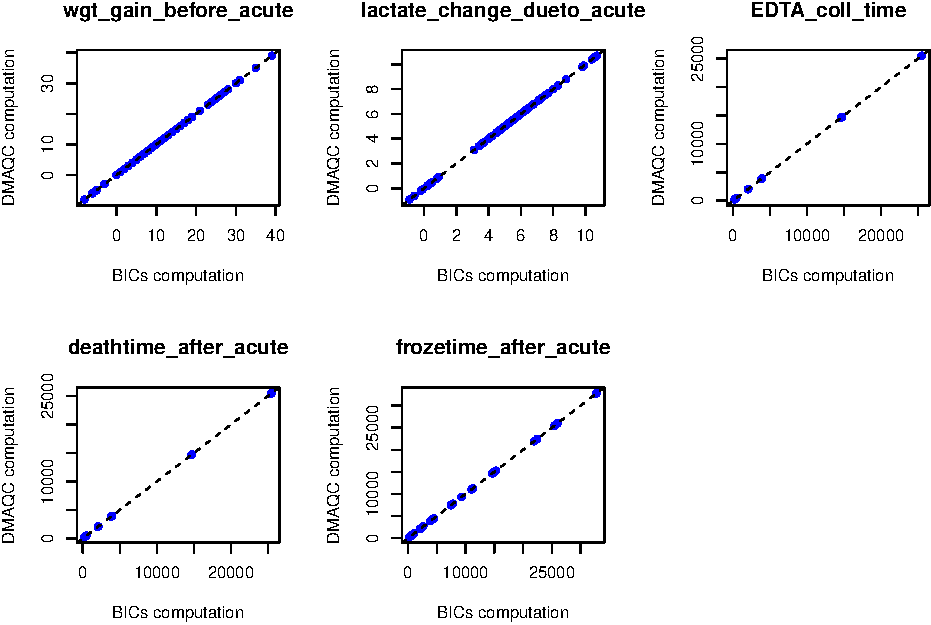
\includegraphics[width=0.9\linewidth,height=0.9\textheight]{pheno_csv_files_analysis_files/figure-latex/unnamed-chunk-7-1} \end{center}

\section{Correlations with time
points}\label{correlations-with-time-points}

Based on the analyses above we know that the distances are mostly
correlated with the shock length and weight/sex. We now plot the
achieved distances as a function of the shock data but colored by the
time point of each animal in the exercise group.

\begin{Shaded}
\begin{Highlighting}[]
\KeywordTok{library}\NormalTok{(ggplot2)}
\NormalTok{parse_timepoint<-}\ControlFlowTok{function}\NormalTok{(x)\{}
\NormalTok{  arrs =}\StringTok{ }\KeywordTok{strsplit}\NormalTok{(x,}\DataTypeTok{split=}\StringTok{" "}\NormalTok{)}
\NormalTok{  tps =}\StringTok{ }\KeywordTok{sapply}\NormalTok{(arrs,}\ControlFlowTok{function}\NormalTok{(x)x[}\DecValTok{3}\NormalTok{])}
\NormalTok{  tps =}\StringTok{ }\KeywordTok{as.numeric}\NormalTok{(tps)}
\NormalTok{  tps[}\KeywordTok{is.na}\NormalTok{(tps)]=}\OperatorTok{-}\DecValTok{1}
  \KeywordTok{return}\NormalTok{(tps)}
\NormalTok{\}}

\CommentTok{# colnames(merged_dmaqc_data)[grepl("sex",colnames(merged_dmaqc_data))]}
\NormalTok{merged_dmaqc_data}\OperatorTok{$}\NormalTok{timepoint =}\StringTok{ }\KeywordTok{parse_timepoint}\NormalTok{(merged_dmaqc_data[,}\StringTok{"Animal.Key_ANIRandGroup"}\NormalTok{])}
\end{Highlighting}
\end{Shaded}

\begin{verbatim}
## Warning in parse_timepoint(merged_dmaqc_data[, "Animal.Key_ANIRandGroup"]):
## NAs introduced by coercion
\end{verbatim}

\begin{Shaded}
\begin{Highlighting}[]
\NormalTok{merged_dmaqc_data}\OperatorTok{$}\NormalTok{is_control =}\StringTok{ }\KeywordTok{grepl}\NormalTok{(}\StringTok{"control"}\NormalTok{,}
\NormalTok{      merged_dmaqc_data[,}\StringTok{"Animal.Key_ANIRandGroup"}\NormalTok{],}\DataTypeTok{ignore.case =}\NormalTok{ T)}

\CommentTok{# Reduce the data by label ids to avoid duplications}
\NormalTok{inds =}\StringTok{ }\OperatorTok{!}\KeywordTok{is.na}\NormalTok{(merged_dmaqc_data}\OperatorTok{$}\StringTok{`}\DataTypeTok{Acute.test_howlongshock}\StringTok{`}\NormalTok{)}
\NormalTok{df =}\StringTok{ }\NormalTok{merged_dmaqc_data[inds,}\KeywordTok{c}\NormalTok{(}\StringTok{"bid"}\NormalTok{,}\StringTok{"Acute.test_distance"}\NormalTok{,}
                              \StringTok{"Acute.test_howlongshock"}\NormalTok{,}\StringTok{"timepoint"}\NormalTok{,}
                              \StringTok{"Animal.Registration_sex"}\NormalTok{)]}
\NormalTok{df =}\StringTok{ }\KeywordTok{unique}\NormalTok{(df)}
\KeywordTok{print}\NormalTok{(}\KeywordTok{paste}\NormalTok{(}\StringTok{"Number of bids in the reduced data:"}\NormalTok{,}\KeywordTok{nrow}\NormalTok{(df)))}
\end{Highlighting}
\end{Shaded}

\begin{verbatim}
## [1] "Number of bids in the reduced data: 72"
\end{verbatim}

\begin{Shaded}
\begin{Highlighting}[]
\CommentTok{# Marginal correlation}
\NormalTok{rho =}\StringTok{ }\KeywordTok{cor}\NormalTok{(df}\OperatorTok{$}\StringTok{`}\DataTypeTok{Acute.test_howlongshock}\StringTok{`}\NormalTok{,}
\NormalTok{          df}\OperatorTok{$}\StringTok{`}\DataTypeTok{Acute.test_distance}\StringTok{`}\NormalTok{)}
\NormalTok{rho =}\StringTok{ }\KeywordTok{format}\NormalTok{(rho,}\DataTypeTok{digits =} \DecValTok{3}\NormalTok{)}

\CommentTok{# A simple 2D plot}
\KeywordTok{ggplot}\NormalTok{(df,}
       \KeywordTok{aes}\NormalTok{(}\DataTypeTok{x=}\StringTok{`}\DataTypeTok{Acute.test_distance}\StringTok{`}\NormalTok{, }\DataTypeTok{y=}\StringTok{`}\DataTypeTok{Acute.test_howlongshock}\StringTok{`}\NormalTok{,}
           \DataTypeTok{shape=}\KeywordTok{as.factor}\NormalTok{(Animal.Registration_sex), }\DataTypeTok{color=}\KeywordTok{as.factor}\NormalTok{(timepoint))) }\OperatorTok{+}\StringTok{ }
\StringTok{  }\KeywordTok{geom_point}\NormalTok{(}\DataTypeTok{size=}\DecValTok{2}\NormalTok{) }\OperatorTok{+}\StringTok{ }\KeywordTok{ggtitle}\NormalTok{(}\KeywordTok{paste}\NormalTok{(}\StringTok{"Distance vs. Shock length (+time point), rho="}\NormalTok{,rho)) }\OperatorTok{+}\StringTok{ }
\StringTok{  }\KeywordTok{theme}\NormalTok{(}\DataTypeTok{plot.title =} \KeywordTok{element_text}\NormalTok{(}\DataTypeTok{hjust =} \FloatTok{0.5}\NormalTok{))}
\end{Highlighting}
\end{Shaded}

\begin{center}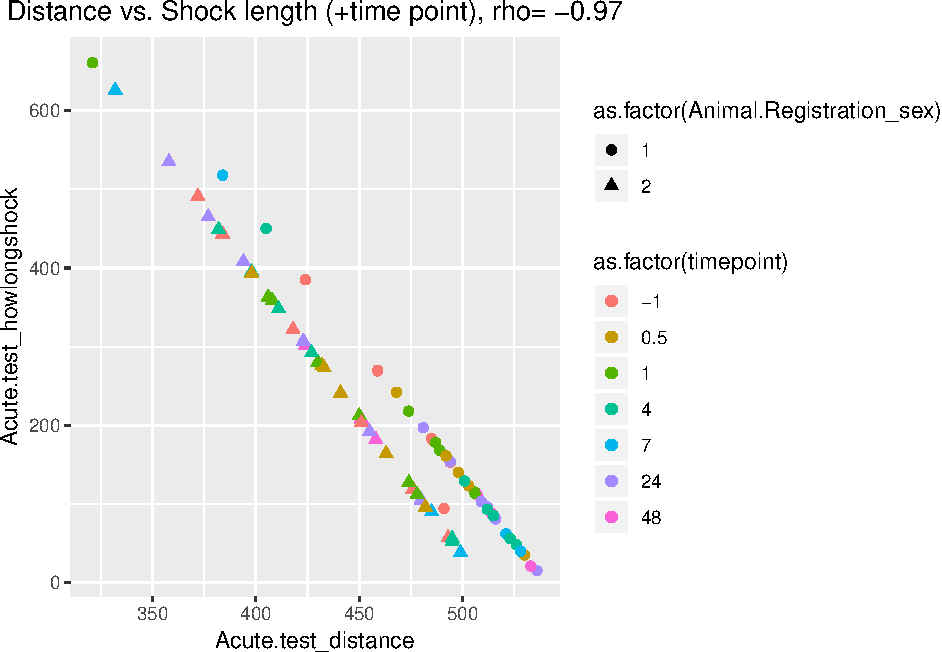
\includegraphics[width=0.6\linewidth,height=0.6\textheight]{pheno_csv_files_analysis_files/figure-latex/unnamed-chunk-8-1} \end{center}

\begin{Shaded}
\begin{Highlighting}[]
\CommentTok{# Look at the linear regression, do we see a correlation between time}
\CommentTok{# and distance?}
\NormalTok{dist_lm2 =}\StringTok{ }\KeywordTok{lm}\NormalTok{(Acute.test_distance}\OperatorTok{~}\NormalTok{Acute.test_howlongshock}\OperatorTok{+}
\StringTok{                }\KeywordTok{as.factor}\NormalTok{(timepoint)}\OperatorTok{+}\NormalTok{Animal.Registration_sex,}\DataTypeTok{data=}\NormalTok{df)}
\KeywordTok{print}\NormalTok{(}\StringTok{"No significant linear association between the time points and distance:"}\NormalTok{)}
\end{Highlighting}
\end{Shaded}

\begin{verbatim}
## [1] "No significant linear association between the time points and distance:"
\end{verbatim}

\begin{Shaded}
\begin{Highlighting}[]
\KeywordTok{summary}\NormalTok{(dist_lm2)}
\end{Highlighting}
\end{Shaded}

\begin{verbatim}
## 
## Call:
## lm(formula = Acute.test_distance ~ Acute.test_howlongshock + 
##     as.factor(timepoint) + Animal.Registration_sex, data = df)
## 
## Residuals:
##      Min       1Q   Median       3Q      Max 
## -19.7934  -0.4604   0.6045   1.3591   5.7995 
## 
## Coefficients:
##                           Estimate Std. Error t value Pr(>|t|)    
## (Intercept)             562.059277   1.806668 311.103   <2e-16 ***
## Acute.test_howlongshock  -0.296516   0.003231 -91.770   <2e-16 ***
## as.factor(timepoint)0.5   1.901423   1.599209   1.189    0.239    
## as.factor(timepoint)1    -0.134233   1.589311  -0.084    0.933    
## as.factor(timepoint)4     2.088966   1.595693   1.309    0.195    
## as.factor(timepoint)7     1.711643   1.947389   0.879    0.383    
## as.factor(timepoint)24    2.571109   1.591651   1.615    0.111    
## as.factor(timepoint)48    1.929356   1.971338   0.979    0.331    
## Animal.Registration_sex -25.134776   0.971100 -25.883   <2e-16 ***
## ---
## Signif. codes:  0 '***' 0.001 '**' 0.01 '*' 0.05 '.' 0.1 ' ' 1
## 
## Residual standard error: 3.893 on 63 degrees of freedom
## Multiple R-squared:  0.9949, Adjusted R-squared:  0.9943 
## F-statistic:  1538 on 8 and 63 DF,  p-value: < 2.2e-16
\end{verbatim}

\section{Save the merged datasets in the
cloud}\label{save-the-merged-datasets-in-the-cloud}

\begin{Shaded}
\begin{Highlighting}[]
\CommentTok{# To see the bucket list}
\CommentTok{# gsutil ls -p motrpac-portal-dev}
\KeywordTok{write.table}\NormalTok{(merged_dmaqc_data,}\DataTypeTok{file=}\StringTok{"merged_dmaqc_data.txt"}\NormalTok{,}\DataTypeTok{quote =}\NormalTok{ F,}\DataTypeTok{sep=}\StringTok{"}\CharTok{\textbackslash{}t}\StringTok{"}\NormalTok{,}\DataTypeTok{row.names =}\NormalTok{ F)}
\KeywordTok{save}\NormalTok{(merged_dmaqc_data,}\DataTypeTok{file=}\StringTok{"merged_dmaqc_data.RData"}\NormalTok{)}
\KeywordTok{system}\NormalTok{(}\StringTok{"gsutil cp merged_dmaqc_data.txt gs://bic_data_analysis/pass1a/pheno_dmaqc/"}\NormalTok{)}
\end{Highlighting}
\end{Shaded}


\end{document}
